\documentclass[conference]{IEEEtran}

\title{Finding Optimal Solutions \\ for Alternative Feature Selection}
\author{
	\IEEEauthorblockN{Jakob Bach}
	\IEEEauthorblockA{
		\textit{Department of Informatics} \\
		\textit{Karlsruhe Institute of Technologie (KIT)}\\
		Karlsruhe, Germany \\
		jakob.bach@kit.edu
	}
}

% \usepackage[style=ieee, backend=bibtex]{biblatex}; handled by IEEE template
\usepackage[tworuled, linesnumbered,vlined]{algorithm2e} % pseudo-code; use of package discouraged by IEEE, but hacked in in a (hopefully acceptable) way
\usepackage{amsmath} % mathematical symbols
\usepackage{amssymb} % mathematical symbols
\usepackage{amsthm} % theorems, definitions etc.
\usepackage{balance} % balance columns on the last page
\usepackage{graphicx} % plots
\usepackage[caption=false,font=footnotesize]{subfig} % figures with multiple sub-figures and sub-captions; use of (newer) package "subcaption" discouraged by IEEE
\usepackage{hyperref} % links and URLs
%\addbibresource{references.bib}; handled by IEEE template

\theoremstyle{definition}
\newtheorem{definition}{Definition}

\begin{document}

\maketitle

\begin{abstract}
Feature-selection methods are popular to obtain small, interpretable, yet highly accurate prediction models.
Existing feature-selection methods typically yield only one feature set, which might not be sufficient in some cases.
For example, users might be interested in finding different feature sets with similar prediction quality, offering alternative explanations of the data.
In this article, we formalize alternative feature selection as optimization problem.
Next, we propose several general approaches to solve this problem.
In particular, we show how to integrate various categories of existing feature-selection methods.
Finally, we evaluate these approaches in a study with 30 classification datasets.
In our experiments, we are able to determine alternative feature sets with high prediction quality.
\end{abstract}

\begin{IEEEkeywords}
feature selection, alternatives, constraints, explainability, interpretability
\end{IEEEkeywords}

\section{Introduction}
\label{sec:introduction}

\paragraph{Motivation}

Feature-selection methods are ubiquitous for various reasons.
By reducing dataset dimensionality, they lower computational and memory requirements of prediction models.
Next, models might generalize better if irrelevant and spurious predictors are removed.
Finally, prediction models might be smaller and more comprehensive due to feature selection~\cite{li2017feature}, improving interpretability.

Traditional feature-selection methods mostly return only one feature set~\cite{borboudakis2021extending}.
These methods optimize a criterion of feature-set quality, e.g., prediction performance.
However, besides the optimal feature set, there might be other, differently composed feature sets with similar quality.
For the user, these alternative feature sets might be interesting for multiple reasons.
First, some of the originally selected features might be costly to obtain, so the user would prefer cheaper alternatives.
Second, some of the originally selected features might contain sensitive information that should not be used in predictions.
Third, the user might be interested in explanations for the prediction.
In such a situation, knowing alternatives allows formulating multiple hypotheses and broadens the understanding.

\paragraph{Problem statement}

This article addresses the problem of alternative feature selection, which we define as follows:
%
\begin{definition}[Alternative feature selection (informal)]
	Given an original feature set, find a sufficiently different feature set that optimizes feature-set quality at the same time.
	\label{def:alternative-feature-selection}
\end{definition}
%
We provide formal definitions later.
If the original feature set had high quality, the alternative feature set should have similar quality.
Depending on how different the alternative should be, one might have to compromise on quality.
E.g., if original feature set already contains most of the highly predictive features, the alternative might have significantly lower quality.
We analyze this effect in our article.
Also, we consider finding multiple alternatives rather than just one.

Two points are essential for alternative feature selection, which we both address in this article.
First, one needs to formalize and quantify what an alternative feature sets is.
Second, one needs an approach to efficiently find alternative feature sets.
Ideally, the approach should be general, i.e., cover a broad range of existing feature-selection methods.

\paragraph{Related work}

In machine learning, finding alternative solutions has already been addressed extensively in clustering~\cite{bailey2014alternative}.
However, there is a lack of such approaches and corresponding experimental evaluation for feature selection.
Only few feature-selection methods target at obtaining multiple, diverse feature sets~\cite{borboudakis2021extending, siddiqi2020genetic}.
Techniques for ensemble feature selection~\cite{saeys2008robust, seijo2017ensemble} and statistically equivalent feature subsets~\cite{lagani2017feature} produce multiple feature sets, but do not focus on optimal alternatives.
In the field of explainable AI, counterfactual explanations have massively gained popularity in the last few years~\cite{verma2020counterfactual, stepin2021survey}.
Such explanations involve data objects with similar feature values, but a different prediction outcome.
In contrast, we target at sets of different features, but similar feature-set quality, e.g., prediction performance.

\paragraph{Contributions}

Our contribution is threefold.
First, we formalize alternative feature selection as an optimization problem.
In particular, we foster alternatives via constraints on feature sets.
Second, we propose heuristic and exact approaches to solve this optimization problem.
To that end, we discuss how to integrate different categories of feature-selection methods in the objective function.
Our notion of alternative feature sets is general and thus not tailored towards specific feature-selection methods.
Third, we evaluate our approaches for alternative feature selection with comprehensive experiments.
We use 30 classification dataset from the Penn Machine Learning Benchmarks (PMLB)~\cite{olson2017pmlb, romano2021pmlb} and four different feature-selection methods.
We focus on the question if one can find alternative feature sets with similar feature-set quality as the original ones.

\paragraph{Results}

Our experiments show that finding alternative feature sets with similar feature-set quality is possible.
This outcome encourages using alternative feature sets as a tool for alternative explanations of predictions.
As expected, feature-set quality tends to decrease with the number of alternatives.
Naturally, the exact decrease depends on the dataset and how feature-set quality is distributed in it.
Further, we note that the quality of alternatives significantly depends on the dissimilarity threshold for how alternative feature sets should be.
Thereby, this threshold allows the user to exercise control over alternatives and make use-case specific choices.

We publish our code\footnote{\url{https://github.com/Jakob-Bach/AFS}} and our experimental data\footnote{temporary link: \url{https://bwsyncandshare.kit.edu/s/xxx}; will be moved to a public repository after review} online.

\paragraph{Outline}

Section~\ref{sec:fundamentals} explains fundamentals of feature selection.
Section~\ref{sec:approach} defines the optimization problem of alternative feature selection and discusses approaches to solve it.
Section~\ref{sec:related-work} reviews related work.
Section~\ref{sec:experimental-design} describes our experimental design.
Section~\ref{sec:evaluation} presents the experimental results.
Section~\ref{sec:conclusion} concludes.

\section{Fundamentals}
\label{sec:fundamentals}

In this section, we introduce basic notation and review different methods to measure quality of feature sets.

\subsection{Notation}
\label{sec:fundamentals:notation}

Let $X \in \mathbb{R}^{m \times n}$ be a dataset represented as a matrix.
Each row is a data object, and each column is a feature.
Let $F = \{f_1, \dots, f_n\}$ denote the set of feature names.
We assume categorical features have already been made numeric, e.g., via one-hot encoding.
Let $X_{\cdot{}j} \in \mathbb{R}^m$ denote the vector representation of the $j$-th feature.
Further, let $y \in \mathbb{R}^m$ represent the prediction target.
The actual domain of the target might also be smaller, e.g., $\{0,1\}$ for binary classification.

With feature selection, one makes a binary decision $s_j \in \{0,1\}$ for each feature, i.e., either selects it or not.
The vector $s \in \{0,1\}^n$ combines all these selection decisions.
The selected feature set is $F_s = \{f_j \mid s_j=1\}$.
Let the function $Q(s,X,y)$ return the quality of a such feature set.
Without loss of generality, we assume this function should be maximized.

\subsection{Measuring Feature (Set) Quality}
\label{sec:fundamentals:quality}

There are different ways to evaluate feature-set quality $Q(s,X,y)$.
Note that we only give a short overview here, and focus on methods that we use in our evaluation.
See~\cite{chandrashekar2014survey,li2017feature} for comprehensive surveys of feature selection.
A typical categorization of feature selection is into filter, wrapper, and embedded methods~\cite{guyon2003introduction}.

\paragraph{Filter methods}

Filter methods evaluate feature sets without training a prediction model.
Univariate filters assess each feature on its own, while multivariate filters evaluate feature sets.
Examples for univariate filters are the Pearson correlation or the mutual information between a feature and the prediction target.
Such methods ignore interaction between features, e.g., redundancies.
Multivariate methods, like CFS~\cite{hall1999correlation}, FCBF~\cite{yu2003feature}, and mRMR~\cite{peng2005feature}, often combine a measure of feature relevance with a measure of feature redundancy to express feature-set quality.
%Another interesting filter method is Relief~\cite{kira1992feature}, for which multiple extensions exist.
%While Relief assigns quality to individual features rather than feature sets, it still uses other features indirectly via nearest-neighbor computations between data objects.

\paragraph{Wrapper methods}

Wrapper methods~\cite{kohavi1997wrappers} assess feature-set quality by training a prediction model with the feature set and evaluating prediction performance.
They can use an arbitrary black-box optimization strategy to iterate over feature sets, e.g., genetic algorithms.

\paragraph{Embedded methods}

Embedded methods have feature selection built into training of prediction models, e.g., decision trees~\cite{breiman1984classification} or random forests~\cite{breiman2001random}.
Thus, the criterion to evaluate feature-set quality often is model-specific.
Tree-based models typically use information gain or the Gini index.

\paragraph{Post-hoc feature-importance methods}

Apart from traditional feature selection, there are various methods that assess feature importance after training a model.
Assessing feature importance plays a crucial role in the emerging fields of ML interpretability~\cite{carvalho2019machine}.
Approaches range from local explanation methods, like LIME~\cite{ribeiro2016should} or SHAP~\cite{lundberg2017unified}, to global importance methods, like permutation importance~\cite{breiman2001random} or SAGE~\cite{covert2020understanding}.

\section{Alternative Feature Selection}
\label{sec:approach}

In this section, we present the problem and approaches for alternative feature selection.
First, we give an overview of the optimization problem.
Second, we formalize the notion of alternatives via constraints.
Third, we discuss different objective functions, corresponding to different feature-set quality measures from Section~\ref{sec:fundamentals:quality}
In particular, we describe how to solve the resulting the optimization problem.

\subsection{Optimization Problem}
\label{sec:approach:problem}

In alternative feature selection, there are two goals.
First, the quality of an alternative feature set should be high.
Second, an alternative feature set should be different to one or more existing feature set(s).
There are different ways to combine these two goals in an optimization problem:

First, one can consider both goals as objectives, obtaining an unconstrained multi-objective problem.
Second, one can treat feature-set quality as objective and enforce alternatives with constraints.
Third, one can consider being alternative as objective and constrain feature-set quality, e.g., with a lower bound.
Fourth, one can define constraints for both, feature-set quality and being alternative, searching for feasible solutions instead of optimizing.
Depending on the use case, any of these four formulations might be appropriate.

Following the informal Definition~\ref{def:alternative-feature-selection} from the introduction, we stick to the second formulation, i.e., optimizing feature-set quality subject to being alternative.
This option has the advantage of keeping the original objective function of feature selection.
Consequently, one does not need to specify a range or a threshold on feature-set quality.
Instead, the user can control how alternative the feature set should be.
This yields the following optimization problem:
%
\begin{equation}
	\begin{split}
	\max_s & \quad Q(s,X,y) \\
	\text{subject to:} & \quad F_s~\text{being alternative}
	\end{split}
\label{eq:afs}
\end{equation}
%
We discuss different constraints for \emph{being alternative} and different objective functions $Q(s,X,y)$ in the following.

\subsection{Constraints -- Defining Alternative Feature Sets}
\label{sec:approach:constraints}

In this section, we formalize alternative feature sets.
This part our work is independent from the feature-selection method.
First, we discuss the base case where an individual feature set is an alternative to another one.
Second, we extend this notion to multiple alternatives, considering sequential as well as simultaneous search procedures.

\subsubsection{Single Alternatives}
\label{sec:approach:constraints:single}

We consider a feature set to be an alternative to another feature set if it differs sufficiently.
Mathematically, we express this with a set-dissimilarity measure~\cite{egghe2009new}.
Most of these measures describe how strongly two sets overlap and set this in relation to the size of the sets.
For example, one can define dissimilarity based on the Dice coefficient, a simple and well-known set-similarity measure:
%
\begin{equation}
	d_{Dice}(F_1,F_2) = 1 - \frac{2 \cdot |F_1 \cap F_2|}{|F_1| + |F_2|}
	\label{eq:dice}
\end{equation}
%
% %
% \begin{equation}
%	begin{aligned}
%	d_{Jacc}(F_1,F_2) & = 1 - \frac{|F_1 \cap F_2|}{|F_1 \cup F_2|} \\
%	& = 1 - \frac{|F_1 \cap F_2|}{|F_1| + |F_2| - |F_1 \cap F_2|}
%	\end{aligned}
%	\label{eq:jaccard}
%\end{equation}
% %
We leverage such a set-dissimilarity measure for the following definition:
%
\begin{definition}[Pairwise alternative]
	A feature set $F_2$ is an alternative to a feature set $F_1$ (and vice versa) for a dissimilarity threshold $\tau \in [0,1]$ if $d(F_1,F_2) \geq \tau$.
	\label{def:single-alternative}
\end{definition}
%
Depending on the preferences of the user, different values of $\tau$ might be appropriate.
$\tau$ controls how alternative the new feature set should be.
A feature set that differs strongly might cause a large drop in feature-set quality.
Thus, we leave $\tau$ as a parameter.
If the set-dissimilarity measure $d()$ is normalized to $[0,1]$, like the Dice dissimilarity, the interpretation of $tau$ is user-friendly:
A value of $0$ allows the alternative feature set to be identical to the original feature set.
A value of $1$ requires the two feature sets to have no overlap.

If the feature sets sizes $|F_1|$ and $|F_2|$ are known, a threshold $\tau$ corresponds to a particular maximum number of overlapping features $|F_1 \cap F_2|$.
This follows from re-arranging Equation~\ref{eq:dice} in combination with Definition~\ref{def:single-alternative}:
%
\begin{equation}
	d_{Dice}(F_1,F_2) \geq \tau \Leftrightarrow |F_1 \cap F_2| \leq \frac{1 - \tau}{2} \cdot (|F_1| + |F_2|)
	\label{eq:dice-rearranged}
\end{equation}
%
%%
%\begin{equation}
%	\begin{aligned}
%	d_{Jacc}(F_1,F_2) & = 1 - \frac{|F_1 \cap F_2|}{|F_1| + |F_2| - |F_1 \cap F_2|} \geq \tau \\
%	& \Leftrightarrow |F_1 \cap F_2| \leq \frac{1 - \tau}{2 - \tau} \cdot (|F_1| + |F_2|)
%	\end{aligned}
%	\label{eq:jaccard-rearranged}
%\end{equation}
%%
The latter formulation also avoids having the feature-set sizes, and thereby the decision variables, in a quotient.
We can see that the effect of setting $\tau$ on the maximum overlap size $|F_1 \cap F_2|$ is linear.
For the Jaccard distance, another popular set-dissimilarity measure, we would obtain a non-linear expression regarding $\tau$.

If we additionally require $|F_1| = |F_2|$, the parameter $\tau$ directly controls which fraction of features in one set needs to differ from the other set, and vice versa:
%
\begin{equation}
	\begin{aligned}
	\text{If}~|F_1| = |F_2|: \quad d_{Dice}(F_1,F_2) \geq \tau \\
	\Leftrightarrow |F_1 \cap F_2| \leq (1 - \tau) \cdot |F_1| = (1 - \tau) \cdot |F_2|
	\end{aligned}
\end{equation}
%
Up to now, we have worked with feature set sizes instead of the binary feature-selection vector $s$.
However, expressing the feature-set sizes in terms of $s$ is straightforward:
%
\begin{equation}
	|F_s| = \sum_{j=1}^n s_j \quad \text{and} \quad |F_{s_1} \cap F_{s_2}| = \sum_{j=1}^n s_{1,j} \cdot s_{2,j}
	\label{eq:feature-set-size}
\end{equation}
%
Combining Equation~\ref{eq:dice-rearranged} with Equation~\ref{eq:feature-set-size} yields an inequality only involving sums and products of the decision variables and constants.
In fact, one can replace the product $s_{1,j} \cdot s_{2,j}$ with linear constraints by introducing an auxiliary variable $t_j$~\cite{mosek2021modeling}:
%
\begin{equation}
	\begin{aligned}
	t_j \leq& s_{1,j} & t_j \leq& s_{2,j} \\
	1 + t_j \geq& s_{1,j} + s_{2,j} & t_j \in& \{0,1\}
	\end{aligned}
	\label{eq:product-linear}
\end{equation}
%
If there is an existing feature set, i.e., one either knows $s_1$ or $s_2$, Equation~\ref{eq:feature-set-size} already is linear without Equation~\ref{eq:product-linear}.

Overall, one can express alternative features sets according to Definition~\ref{def:single-alternative} with 0-1 integer linear constraints.
This simple constraint type allows using a broad range of solvers, given the right objective function, which we discuss later.

\subsubsection{Multiple Alternatives}
\label{sec:approach:constraints:multiple}

If the user desires multiple alternative feature sets rather than just one, one can compute these alternatives either sequentially or simultaneously.

\paragraph{Sequential alternatives}

In the sequential case, we obtain alternatives iteratively, with one alternative feature set per iteration.
We constrain the new feature set to be alternative to all previously found feature sets:
%
\begin{definition}[Sequential alternative]
	A feature set $F_2$ an alternative to a set of feature sets $\mathbb{F}$ (and vice versa) for a dissimilarity threshold $\tau \in [0,1]$ if $\forall F_1 \in \mathbb{F}: d(F_1,F_2) \geq \tau$.
	\label{def:sequential-alternative}
\end{definition}
%
This definition duplicates the constraint from the base case and instantiates it for different existing feature sets.
One could also use a less strict constraint, e.g., requiring only the average dissimilarity to all existing feature sets to pass the threshold.
The objective function remains the same as in the base case, i.e., we only optimize the quality of the new feature set~$F_2$.
Thus, the number of variables in the optimization problem remains constant, independent from the number of alternatives.
Further, we do not need to introduce interaction variables as in Equation~\ref{eq:product-linear}.
Each alternative only adds one new constraint to the optimization problem.
Thus, we expect the runtime of sequential search to scale well with the number of alternatives.
If the solver keeps a state between iterations and can warm-start, further runtime gains might be possible.
Regarding feature-set quality, one can expect a drop with each alternative, as the solution space becomes narrower over iterations.
The user can decide after each iteration if feature-set quality is too low or if another alternative should be found.

\paragraph{Simultaneous alternatives}

In the simultaneous case, we directly obtain several alternatives.
The user needs to decide on the number of feature sets $\mathbb{F}$ beforehand.
This entails pairwise dissimilarity constraints:
%
\begin{definition}[Simultaneous alternatives]
	A set of feature sets $\mathbb{F}$ contains pairwise alternatives for a dissimilarity threshold $\tau \in [0,1]$ if $\forall F_1 \in \mathbb{F}, F_2 \in \mathbb{F}, F_1 \neq F_2: d(F_1,F_2) \geq \tau$.
	\label{def:simultaneous-alternative}
\end{definition}
%
Again, one could resort to less strict constraints, e.g., based on the average dissimilarity between alternatives.
In contrast to the sequential case, we need to introduce further decision variables and modify the objective function here, as we optimize multiple feature sets at once.
In this paper, we consider the summed quality of all feature sets as objective.

Runtime-wise, we expect simultaneous search to scale worse with the number of alternatives than sequential search.
The number of decision variables increases linearly with the number of alternatives, while the number of constraints grows quadratically.
Also, for each feature and each pair of alternatives, we need to introduce an interaction variable as in Equation~\ref{eq:product-linear} if we want to obtain a linear problem.

In contrast to the greedy procedure of the sequential procedure, the simultaneous procedure optimizes alternatives globally.
Thus, for the same number of alternatives, the simultaneous procedure should yield higher average feature-set quality.
Also, we expect the qualities of the alternatives to be more evenly distributed, opposed to the dropping quality over the course of the sequential procedure.

\subsection{Objective Functions -- Finding Alternative Feature Sets}
\label{sec:approach:objectives}

In this section, we present concrete approaches to find alternative feature sets.
We discuss how to solve the optimization problem from Section~\ref{sec:approach:problem} for the different categories of feature-set quality measures from Section~\ref{sec:fundamentals:quality}.
In particular, we categorize solution approaches as white-box optimization, black-box optimization, and embedding alternatives.

\subsubsection{White-Box Optimization}
\label{sec:approach:objectives:white-box}

If feature-set quality~$Q(s,X,y)$ is a sufficiently simple function, one can tackle alternative feature selection with a white-box solver.

\paragraph{Univariate filter feature selection}

For univariate filter feature selection, the objective function is linear.
This makes the optimization problem of alternative feature selection an 0-1 integer linear problem.
In particular, univariate filter methods decompose the quality of a feature set into the quality of the individual features:
%
\begin{equation}
	Q_{uni}(s,X,y) = \sum_{j=1}^{n} s_j  \cdot q(X_{\cdot{}j},y)
	\label{eq:univariate-filter}
\end{equation}
%
Here, $q$ typically is a bivariate dependency measure, e.g., mutual information~\cite{kraskov2004estimating} or correlation, to quantify the relationship between a feature and the prediction target.

\paragraph{Post-hoc feature importance}

From the technical perspective, one can also insert values of post-hoc feature importance scores for $q$ in Equation~\ref{eq:univariate-filter}.
For example, one can pre-compute permutation importance~\cite{breiman2001random} or SAGE scores~\cite{covert2020understanding} for each feature.
However, such post-hoc importance scores often evaluate the usefulness of features under the presence of other features.
In consequence, the feature-independence assumption underlying Equation~\ref{eq:univariate-filter} does not hold.
However, re-calculating feature importance for each possible feature set makes a white-box approach infeasible.
In practice, one can still use Equation~\ref{eq:univariate-filter} with importance scores computed on the full dataset.
One only needs to be aware that such an approach might not represent feature interactions faithfully.

\paragraph{Multivariate filter feature selection}

Several multivariate filter methods also enable a simple white-box formulation, though not necessarily a linear one.
In the following, we discuss the Fast Correlation-Based Filter (FCBF)~\cite{yu2003feature}, which we use in our experiments.
Correlation-based Feature Selection (CFS)~\cite{hall1999correlation} and Minimal Redundancy Maximum Relevance (mRMR)~\cite{peng2005feature} allow white-box optimization~\cite{nguyen2014effective} as well.

%\paragraph{CFS}
%
%Correlation-based Feature Selection (CFS)~\cite{hall1999correlation} considers both relevance and redundancy of features.
%Relevance is the correlation between features and prediction target, similar to the univariate filter.
%Redundancy is the correlation between features, acting as a normalization term.
%Using a bivariate dependency measure $q$ to quantify correlation, the objective is as follows:
%%
%\begin{multline}
%	Q_{CFS}(s,X,y) = \\
%	\frac{\sum_{j=1}^{n} s_j \cdot q(X_{\cdot{}j},y)}{\sqrt{\sum_{j=1}^{n} s_j + \sum_{j_1=1}^{n} \sum_{\substack{j_2=1 \\ j_2 \neq j_1}}^{n} s_{j_1} \cdot s_{j_2} \cdot q(X_{\cdot{}j_1}, X_{\cdot{}j_2})}}
%	\label{eq:cfs}
%\end{multline}
%%
%\paragraph{mRMR}
%
%Minimal Redundancy Maximum Relevance (mRMR)~\cite{peng2005feature} follows a similar principle as CFS, but uses the difference instead of the ratio between relevance and redundancy:
%%
%\begin{multline}
%	Q_{mRMR}(s,X,y) = \frac{\sum_{j=1}^{n} s_j \cdot q(X_{\cdot{}j},y)}{\sum_{j=1}^{n} s_j} - \\
%	\frac{\sum_{j_1=1}^{n} \sum_{j_2=1}^{n} s_{j_1} \cdot s_{j_2} \cdot q(X_{\cdot{}j_1}, X_{\cdot{}j_2})}{(\sum_{j=1}^{n} s_j)^2}
%	\label{eq:mrmr}
%\end{multline}
%%
%Note that if one knows the feature-set size, he denominators are constant and thus, Equation~\ref{eq:mrmr} is linear if one replaces the product terms according to Equation~\ref{eq:product-linear}.
%Without this replacement, it is a quadratic-programming problem~\cite{rodriguez2010quadratic, nguyen2014effective}.
%
%\paragraph{FCBF}

FCBF~\cite{yu2003feature} bases on the notion of predominance:
It strives to select features that have at least a certain correlation to the prediction target, but a lower correlation to all other features.
While the original FCBF algorithm uses a heuristic search, we propose a formulation as a constrained optimization problem:
%
\begin{equation}
	\begin{aligned}
	\max_s &\quad Q_{FCBF}(s,X,y) = \sum_{j=1}^{n} s_j \cdot q(X_{\cdot{}j},y) \\
	\text{subject to:} &\quad \forall (j_1,j_2) \in \{1, \dots, n\}^2, j_1 \neq j_2: \\
	&\quad s_{j_1} \cdot s_{j_2} \cdot q(X_{\cdot{}j_1}, X_{\cdot{}j_2}) < q(X_{\cdot{}j_1},y)
	\end{aligned}
	\label{eq:fcbf}
\end{equation}
%
We drop the original FCBF's threshold parameter on feature-target correlation and instead maximize the latter, as in the univariate filter case.
With the constraint in Equation~\ref{eq:fcbf}, we enforce that if two feature are selected, their correlation is lower than each feature's target correlation.
Overall, the optimization problem is linear again if one appropriately handles the product term between decision variables.

%\paragraph{Relief}
%
%Relief~\cite{kira1992feature} assigns a score to each features by sampling data objects and considering the difference in feature values compared to their nearest neighbors.
%The idea is that data objects with a similar value of the prediction target should have similar feature values.
%In contrast, data objects that differ in their prediction target should differ in their feature values as well.
%We consider this method multivariate as nearest-neighbor computations involve all features instead of considering features independently.
%However, the resulting scores for each feature can be put into the univariate objective from Equation~\ref{eq:univariate-filter}.
%Also, one can combine Relief with CFS to consider feature redundancy~\cite{hall1999correlation}, which the default Relief does not.

\subsubsection{Black-Box Optimization}
\label{sec:approach:objectives:black-box}

If feature-set quality has not closed-form expression, one can treat it as a black-box function when searching for alternative feature sets.
This applies to the category of wrapper feature selection.
Using search heuristics, one can optimize such black-box functions by systematically iterating over candidate feature sets.

However, search heuristics often assume an unconstrained search space.
For example, they might propose a candidate feature set that is not alternative enough.
We see multiple ways to address this challenge:
First, one can enumerate and evaluate all feature sets satisfying the constraints, which is inefficient.
Second, one can sample valid feature sets, which is not easy if the procedure should sample uniformly~\cite{ermon2012uniform}.
Third, one can formulate a multi-objective problem, so there are no hard constraints on alternatives any more.
Fourth, one can adapt a search heuristic to consider constraints; this is what we describe in the following.

There are several approaches for adapting search heuristics to constraints.
One idea is to prevent a search heuristic from producing feature sets that violate the constraints, or at least making the latter less likely, e.g., be penalizing the objective function accordingly.
Another idea is to `repair' feature sets proposed by the search that are not alternative enough.
For example, one can replace a feature set violating the constraint with the most similar feature set satisfying the constraints.
Such solver-assisted search approaches are common in search procedure for software configuration~\cite{white2010automated,henard2015combining,guo2018preserve}.

As a simple wrapper approach for our experiments, we use a greedy hill-climbing strategy, as displayed in Figure~\ref{al:greedy-wrapper}.
Compared to standard hill-climbing~\cite{kohavi1997wrappers}, our search only evaluates feature sets that satisfy the constraints for alternatives.
First, the algorithm uses a solver to find one solution that is sufficiently alternative.
Next, it tries `swapping' a feature, i.e., selecting the feature if it was deselected or deselecting it if it was selected.
The algorithm applies the solver again to find a solution $s'$ containing this change and satisfying the other constraints.
If such a solution $s'$ exists and its quality $Q(s',X,y)$ improves the current solution, the algorithm continuous from the new solution.
Else, it attempts to swap the next feature.
The algorithm terminates if no swap leads to an improvement or a fixed number of iterations $max\_iters$ is reached.
Each iteration corresponds to a solver call.
This also is an upper bound on the number of prediction models trained.
However, not all solver calls might yield a valid feature set.

% IEEE wants algorithms as figures, not separate floats (as "algorithm2e" does), so we need some hacking: https://tex.stackexchange.com/questions/147598/how-to-use-the-algorithm2e-package-with-ieeetran-class
\begin{figure}[t]
\makeatletter
\let\@latex@error\@gobble
\makeatother
\begin{algorithm}[H]
	\DontPrintSemicolon
	\KwIn{
		Dataset $X$, Prediction target $y$, \newline
		Feature-set quality function $Q(\cdot)$, \newline
		Constraints for alternatives $Cons$, \newline
		Maximum number of iterations $max\_iters$
	}
	\KwOut{Feature-selection decision vector $s$}
	\BlankLine
	$s \leftarrow \text{Solve}(Cons)$ \tcp*{Initial alternative}
	$iters \leftarrow 1$ \tcp*{Number of solver calls}
	\lIf(\tcp*[f]{No alternative}){$s = \emptyset$}{\Return{$\emptyset$}}
	$j \leftarrow 1$ \tcp*{Index to be swapped}
	\While{$iters < max\_iters$ \textbf{and} $j \leq |s|$}{
		$s' \leftarrow \text{Solve}(Cons \cup \{\neg s_j\})$ \tcp*{Swap feature}
		$iters \leftarrow iters + 1$\;
		\If{$s' \neq \emptyset$ \textbf{and} $Q(s',X,y) > Q(s,X,y)$}{
			$s \leftarrow s'$\ \tcp*{Swap if improved}
			$j \leftarrow 1$\;
		}
		\lElse(\tcp*[f]{Try next feature}){$j \leftarrow j + 1$}
	}
	\Return{$s$}
\end{algorithm}
\caption{Constraint-aware greedy wrapper feature selection.}
\label{al:greedy-wrapper}
\end{figure}

\subsubsection{Embedding Alternatives}
\label{sec:approach:objectives:embedding}

If feature selection is embedded into training a prediction model, there is no general approach for finding alternative feature sets.
Instead, one would need to embed the search for alternatives into training as well.
In consequence, approaches for embedding alternatives will be specific to prediction models.
For example, one could prevent decision trees from splitting on a feature if the resulting feature set was too similar to an existing feature set.
We leave the formulation of such approaches open for future work.

\section{Related Work}
\label{sec:related-work}

In this section, we review related work from areas related to alternative feature selection:
alternative clustering, subspace search, feature selection, and counterfactual explanations.
To the best of our knowledge, searching for optimal alternative feature sets is novel.
However, there is literature on optimal alternatives outside the field of feature selection.
Also, there are works on finding multiple, diverse feature sets.

\paragraph{Alternative clustering}

Finding alternative solutions has been addressed extensively in the field of clustering.
\cite{bailey2014alternative} gives a taxonomy of alternative clustering and describes algorithms from different categories of alternative clustering.
Our problem definition in Sections~\ref{sec:approach:problem} and~\ref{sec:approach:constraints} is, on a high level, inspired by the one in~\cite{bailey2014alternative}:
find one or multiple solutions that maximize quality while minimizing similarity.
\cite{bailey2014alternative} also draws the distinction between singular alternatives and multiple alternatives, found sequentially or simultaneously.
Nevertheless, the concrete problem definition for our feature-selection scenario is different.

%Besides constraint-based search for alternatives, they discuss other solution paradigms as well.
%For example, feature selection and data transformation can help to find alternative clusterings~\cite{tao2012novel}.

%Two examples of constrained-based alternative clustering are \emph{COALA}~\cite{bae2006coala} and \emph{MAXIMUS}~\cite{bae2010clustering}.
%COALA~\cite{bae2006coala} is a hierarchical algorithm that imposes \emph{cannot-link constraints} on pairs of data objects:
%Data objects assigned to the same cluster in the original clustering should be assigned to different clusters in the alternative clustering.
%If observing the constraints is infeasible or violates a quality threshold, the algorithms proceeds like unconstrained hierarchical clustering.
%MAXIMUS~\cite{bae2010clustering} employs an integer program to formulates dissimilarity between clusterings, building on the distributions of feature values in clusters.
%The solutions of this problem are not concrete alternative clusterings, but constrain a subsequent clustering procedure.

\paragraph{Subspace search}

Finding multiple feature set plays a role in subspace clustering~\cite{mueller2009relevant, guan2011unified, hu2018subspace} and subspace search~\cite{nguyen20134s, trittenbach2019dimension, fouche2021efficient}.
These approaches strive to improve the results of data-mining algorithms by using subspaces, i.e., feature sets, rather than the full space, i.e., all features.
Some subspace approaches explicitly try to remove redundancy between subspaces~\cite{mueller2009relevant, nguyen20134s} or foster subspace diversity~\cite{trittenbach2019dimension, fouche2021efficient}, which bears some resemble to alternative feature selection.
Nevertheless, these unsupervised scenarios have fundamentally different goals than our approaches for supervised feature selection.

\paragraph{Feature selection}

Most feature-selection methods only yield one solution~\cite{borboudakis2021extending}, though there are some exceptions.
Nevertheless, none of the following approaches explicitly searches for optimal alternatives.
\cite{siddiqi2020genetic} adapts a genetic algorithm to ensure diversity of feature sets by penalizing overlap of feature sets.
\cite{emmanouilidis1999selecting} uses multi-objective genetic algorithms to obtain prediction models that use feature sets of different sizes.
\cite{mueller2021feature} clusters features based on their values and then forms all combinations of picking one feature from each cluster.
\cite{leeuwen2012diverse} presents six strategies to foster diversity in subgroup set discovery, which searches for interesting regions in the data space rather than selecting features.

\paragraph{Ensemble feature selection}

Ensemble feature selection~\cite{saeys2008robust, seijo2017ensemble} runs feature selection on different versions, e.g., samples, of the data, or uses different feature-selection methods.
While fostering diverse feature sets might be a sub-goal, the results of the different feature selectors are combined at the end.
Thus, this focus is different from our ours.
As an example, \cite{woznica2012model} uses clustering and frequent-itemset mining to reduce a set of feature-selection results, obtained on bootstrap samples of the data, to a smaller, yet diverse set.
\cite{liu2019subspace} builds an ensemble prediction model from classifiers trained on different feature sets and uses an evolutionary algorithm that ensures diversity of feature sets.
\cite{guru2018alternative} selects features separately for each class and then combines the results.

\paragraph{Statistically equivalent feature sets}

A subfield of feature selection is the search for statistically equivalent feature sets~\cite{lagani2017feature, borboudakis2021extending}.
These approaches use statistical tests to determine which features or feature sets can be used interchangeably to predict a target.
While equivalent feature sets are related to our notion of alternative feature sets, there are differences as well.
Depending on the configuration of statistical tests, there can be an arbitrary number of equivalent feature sets, without a clear ordering.
Instead, we always provide a fixed number of alternatives.
Rather than striving for equivalence between feature sets, we optimize under constraints.
Our dissimilarity threshold allows to control overlap of feature sets, instead of eliminating all feature redundancies.
Nevertheless, if one wants to definitely prevent selection of certain redundant features or feature sets, one can achieve this with additional constraints in our optimization problem as well.

\paragraph{Constrained feature selection}

There is work on considering various kinds of constraints in feature selection, e.g., for costs~\cite{paclik2002feature}, feature group~\cite{yuan2006model}, or domain-knowledge~\cite{groves2015toward}.
These approaches are orthogonal to our work, as such constraints can be added to our optimization problem as well.

\paragraph{Counterfactual explanations}

Alternative feature selection shares some similarities with the concept of counterfactual explanations for predictions~\cite{verma2020counterfactual, stepin2021survey}.
Counterfactual explanations also provide alternative solutions and might be formulated as optimization problem~\cite{mohammadi2021scaling, karimi2020model}.
In particular, \cite{mothilal2020explaining} presents an approach to find diverse counterfactual explanations.
However, there are crucial differences between counterfactuals and alternative feature sets:
Counterfactual explanations target at predictions on single data objects rather than global predictive quality of features.
Also, counterfactuals want to alter the prediction outcome by changing feature values little, while alternative feature sets should keep the prediction quality while changing the feature set significantly.

\section{Experimental Design}
\label{sec:experimental-design}

In this section, we describe our experimental design.
First, we give a brief overview of its goal and components.
Next, we elaborate on different components of the design in detail.

\subsection{Overview}
\label{sec:experimental-design:overview}

We conduct experiments with 30 binary-classification datasets.
In our evaluation, we mainly focus on the trade-off between feature-set quality and obtaining alternative feature sets.
We compare four feature-selection methods, representing different notions of feature-set quality.
Also, we train prediction models with the resulting feature sets, and analyze prediction performance.
To find multiple alternative feature sets, we consider a simultaneous as well as a sequential approach.
We systematically vary the number of alternatives and the dissimilarity threshold for being alternative.

\subsection{Methods}
\label{sec:experimental-design:approaches}

\subsubsection{Feature Selection (Objective Functions)}
\label{sec:experimental-design:approaches:feature-selection}

To have a diverse set of feature-selection methods, we consider the different categories from Section~\ref{sec:fundamentals:quality}.
We choose four feature selection-methods that are well-known and either parameter-free or easy to parameterize.
See Section~\ref{sec:approach:objectives} for details on the objective function of each method.
One method (\emph{Greedy Wrapper}) requires black-box optimization, while the other three methods have white-box objectives.
As explained in Section~\ref{sec:approach:objectives:embedding}, we do not include an embedded method.

For each feature-selection method, we set the number of selected features to $k \in \{5,10\}$.
This yields small feature sets, fostering interpretability.
In our optimization problem, we can enforce the desired $k$ with a simple constraint.
However, 0.03\% of the feature sets from our evaluation violate their prescribed $k$.
These few outliers originate from various experimental settings, so we could not detect a cause.
As a consequence, we remove the affected search runs of alternatives completely, which constitute 0.12\% of all search runs.

\paragraph{MI}

For univariate filtering, we use Equation~\ref{eq:univariate-filter} with mutual information~\cite{kraskov2004estimating} as dependency measure $q()$.
To improve comparability between datasets and values of $k$, we normalize the qualities such that selecting all features yields a quality of 1 and selecting no feature yields a quality of 0.

\paragraph{FCBF}

As multivariate filter method, we use our constrained formulation of FCBF~\cite{yu2003feature} according to Equation~\ref{eq:fcbf}.
As bivariate quality measure within FCBF, we rely on mutual information again, normalized to sum up to 1.

\paragraph{Greedy Wrapper}

As wrapper method, we employ a greedy hill-climbing strategy according to Algorithm~\ref{al:greedy-wrapper}.
We set $max\_iters$ to 1000.
To evaluate feature-set quality within the wrapper, we choose a decision tree as model and Matthews correlation coefficient (MCC)~\cite{matthews1975comparison} as performance metric.
Also, we apply a stratified 80:20 holdout split to test generalization performance.
Thus, $Q(s,X,y)$ corresponds to the MCC on the 20\% validation part of the data.

\paragraph{Model Gain}

As post-hoc importance measure, we take model-based feature importance provided by \emph{scikit-learn}.
Again, we use a decision tree as model.
There, importance expresses a feature's contribution towards optimizing the split criterion of the tree, which for which we choose information gain, i.e., mutual information.
We plug the importances into Equation~\ref{eq:univariate-filter}, i.e., treat the importances like univariate filter scores.
Note that the interpretation is different, though.
Here, the scores originate from trees involving multiple features, rather than assessing features in isolation.
The model-based importances are normalized to sum up to 1 by default.

\subsubsection{Alternatives (Constraints)}
\label{sec:experimental-design:approaches:alternatives}

We employ \emph{sequential} as well as \emph{simultaneous} search for alternatives, using the corresponding definitions from Section~\ref{sec:approach:constraints:multiple}.
For sequential search, we evaluate 1 to 10 alternatives, while for simultaneous search, we examine 1 to 5 alternatives.
This difference stems from the increased runtime for simultaneous search.
For the dissimilarity threshold $\tau$, we analyze all possible sizes of the overlap, or rather the difference between feature sets.
For $k=5$, this means we consider values of $\tau$ from 0.2 to 1 with a step size of 0.2, corresponding to an overlap of four to zero features.
For $k=10$ we consider values of $\tau$ from 0.1 to 1 with a step size of 0.1.
Naturally, we exclude $\tau = 0$, which would allow returning multiple identical feature sets.

As solver runtime may vary considerably even for optimization problems of the same size, we set a timeout of 60~s on each solver run.
If the solver finishes before the timeout, it either found an optimal solution or proved that no solution exists.
In our evaluation, these two outcomes apply to 94\% of the feature sets.
In the remaining cases, the solver had an error, found a feasible but potentially suboptimal solution, or found no solution though one might exist.

%As a simple \emph{baseline} compared to optimization, we use iterative solving to obtain arbitrary feature sets that satisfy the constraints for being alternative.
%In each iteration, the solver has to return a valid feature set that it did not return in a previous iteration.
%To obtain a large sample, we conduct 100 iterations.
%As we neither know nor influence how the solver chooses these solutions, we consider them to be random.
%However, depending on how the solver obtains them, they might not be uniformly random from the space of valid feature sets.

\subsubsection{Prediction}
\label{sec:experimental-design:approaches:prediction}

As prediction models, we use decision trees~\cite{breiman1984classification} as well as random forests with 100 trees \cite{breiman2001random}.
Both types of models allow to learn complex, non-linear dependencies from the data.
We mostly use default hyperparameters of the models, apart from choosing information gain as split criterion and setting a random seed for reproducibility.

Note that tree models carry out feature selection themselves, i.e., they are embedded approaches.
Thus, they need not use all features that we provide to them.
However, this is no problem for our study.
We are interested which performance the models achieve if they are limited to small alternative feature sets, not how they use each feature from an alternative.

\subsection{Evaluation Metrics}
\label{sec:experimental-design:evaluation}

We use two kinds of metrics for feature-set quality.
First, we evaluate the objective functions of the feature-selection methods, which guided the search for feature sets.
Second, we train predictions models with the found feature sets.
We report prediction performance in terms of the Matthews correlation coefficient (MCC), which is insensitive to class imbalance.
This coefficient reaches its maximum of 1 for perfect predictions, and is 0 for random guessing.

To analyze generalization, we conduct stratified 10-fold cross-validation.
Not only model training, but also the search for alternative feature sets is limited to the training data.

\subsection{Datasets}
\label{sec:experimental-design:datasets}

We evaluate alternative feature selection on a variety of datasets from the Penn Machine Learning Benchmarks (PMLB)~\cite{olson2017pmlb,romano2021pmlb}.
To focus the evaluation on one machine-learning task, we only consider binary-classification datasets.
However, alternative feature selection is possible for regression and multi-class problems as well.
We filter out datasets containing less than 100 instances.
Also, we filter out datasets with less than 15 features, to leave some room for alternatives.
Next, we remove one dataset with 1000 features, which would dominate the overall runtime of the experiments.
Finally, we manually remove datasets that seem to be duplicates or modified versions of other datasets from the benchmark.

In consequence, we obtain 30 datasets.
The number of data objects varies from 106 to 9822, and the number of features ranges from 15 to 168.
The datasets contain no missing values.
Categorical features have an ordinal encoding by default.

\subsection{Implementation}
\label{sec:experimental-design:implementation}

We implement our experiments in Python.
For machine learning, we use \emph{scikit-learn}~\cite{pedregosa2011scikit-learn}.
To express and solve the constraint optimization problems, we use \emph{Python-MIP}~\cite{python-mip}.

\section{Evaluation}
\label{sec:evaluation}

In this section, we evaluate our experiments.
In particular, we discuss results for the different dimensions of our experimental design:
datasets, prediction models, feature-selection methods, and approaches to search for alternatives.

\subsection{Datasets}

Naturally, feature-set quality depends on the dataset.
For example, distribution of feature-set quality in datasets might be relatively uniform or relatively skewed.
Datasets with more features $n$ generally allow for more alternative feature sets.
At the same time, the (normalized) feature quality $q(X_{\cdot{}j},y)$ can be spread over more features than for smaller datasets, making it harder to compose a high-quality feature set.

Indeed, our experiments show a broad variation of feature-set quality over datasets.
Further, we do not observe a clear relationship between dimensionality $n$ and feature-set quality.

\subsection{Prediction Models}

\begin{figure}[t]
	\centering
	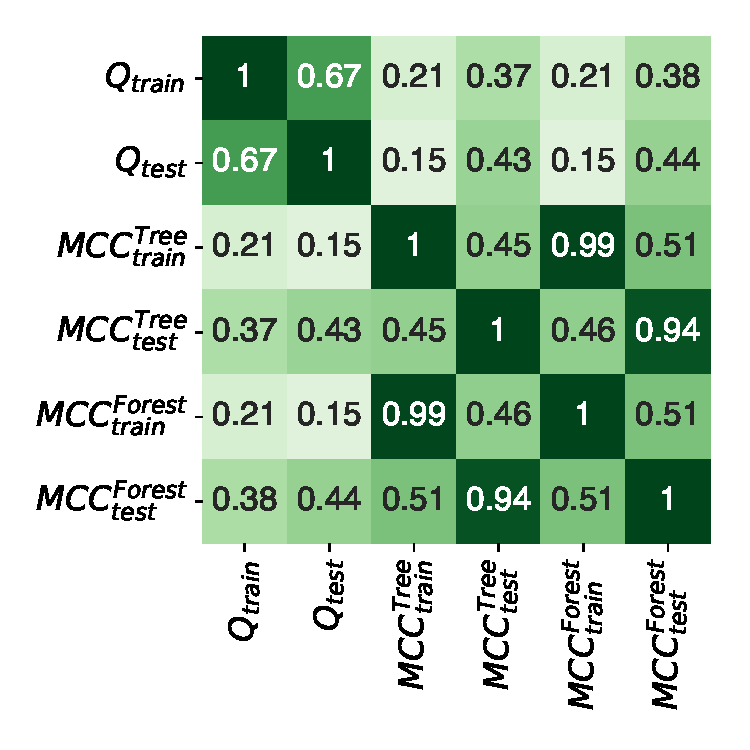
\includegraphics[width=0.7\columnwidth, trim=0 20 0 15, clip]{plots/evaluation-metrics-correlation.pdf}
	\caption{Correlation between evaluation metrics over all experimental settings.}
	\label{fig:evaluation-metrics-correlation}
\end{figure}

\begin{figure*}[t]
	\centering
	\subfloat[Standard deviation of objective.]{
		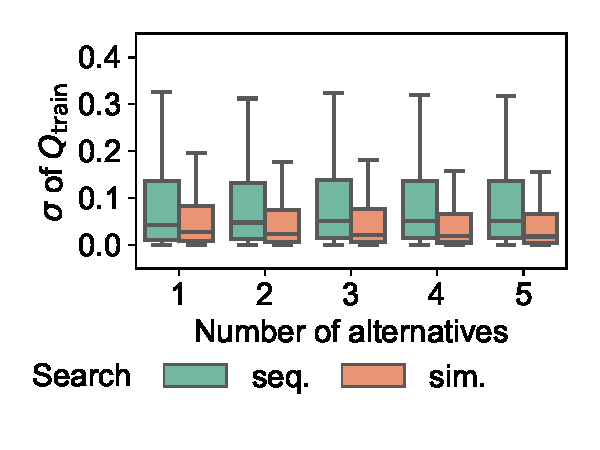
\includegraphics[width=0.99\columnwidth, trim=0 25 0 15, clip]{plots/impact-search-stddev-objective.pdf}
		\label{fig:impact-search-stddev-objective}
	}
	\hfill
	\subfloat[Mean objective.]{
		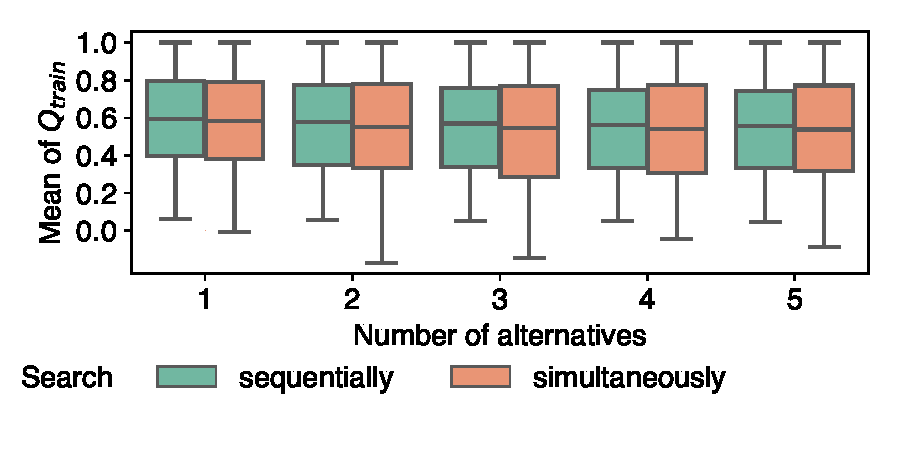
\includegraphics[width=0.99\columnwidth, trim=0 25 0 15, clip]{plots/impact-search-mean-objective.pdf}
		\label{fig:impact-search-mean-objective}
	}
	\caption{Training-set objective value $Q$ in experimental runs of sequential or simultaneous search.
		Outliers removed for readability reasons.}
	\label{fig:impact-search-objective}
\end{figure*}

\begin{figure*}[t]
	\centering
	\subfloat[Max-normalization.]{
		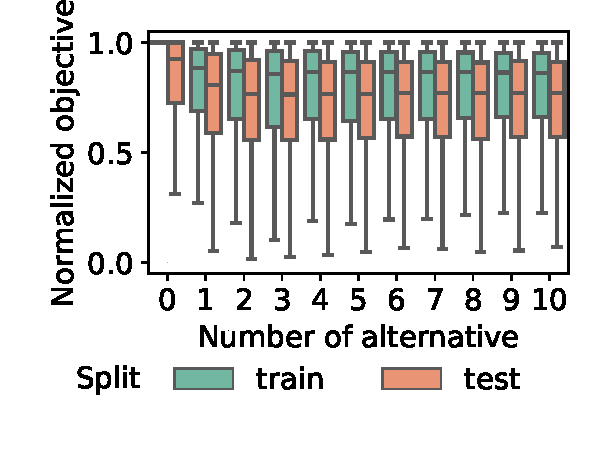
\includegraphics[width=0.99\columnwidth, trim=0 25 0 5, clip]{plots/impact-num-alternatives-objective-max.pdf}
		\label{fig:impact-num-alternatives-objective-max}
	}
	\hfill
	\subfloat[Min-max-normalization.]{
		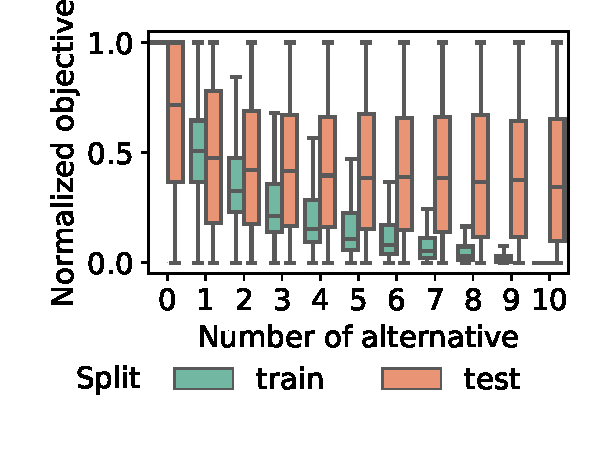
\includegraphics[width=0.99\columnwidth, trim=0 25 0 5, clip]{plots/impact-num-alternatives-objective-min-max.pdf}
		\label{fig:impact-num-alternatives-objective-min-max}
	}
	\caption{Objective value $Q$, normalized per experimental setting, in sequential search, using \emph{MI} as feature selector.
		Outliers removed for readability reasons.}
	\label{fig:impact-num-alternatives-objective}
\end{figure*}

As one can expect, the average prediction performance of random forests is higher than for decision trees.
Also, overfitting occurs for both models, i.e., there is a gap between training-set and test-set prediction performance.
As we do not limit the growth of trees or prune them after training, this observation is expected.
However, that will not prevent our analysis how prediction performance develops over alternative feature sets, where we normalize feature-sets quality.
To a lesser extent, the optimization objective $Q$ also shows overfitting for all feature-selection methods.

Figure~\ref{fig:evaluation-metrics-correlation} shows the Spearman correlation between different evaluation metrics.
As the performance of decision trees and random forests is highly correlated, we focus on decision trees in the following, which always consider all features rather than randomly subsampling them.

Figure~\ref{fig:evaluation-metrics-correlation} also shows that the correlation between training-set quality and test-set quality is moderate, but not high, for the optimization objective $Q$ as well as prediction performance in terms of MCC.
This observation might be an effect of overfitting.
Further, the correlation between $Q$ and MCC is only weak to moderate.
This means that the quality criterion of feature selection is only partially indicative of prediction performance.
In particular, only one of our four feature-selection methods uses prediction performance to assess feature sets.

\subsection{Feature-Selection Methods}

As the different feature-selection methods have different objective functions, it does not make sense to compare objective values between them.
For the optimization status, we note that 89\% of feature sets for \emph{FCBF} could not be determined, as the solver timed out or the optimization problem was infeasible.
For MI, this figure only is 19\%.
In particular, the additional constraints in our formulation of \emph{FCBF} (c.f.~Equation~\ref{eq:fcbf}) seemingly made it hard to find valid feature sets.

Regarding test-set prediction performance, \emph{Model Gain} is best on average.
The median test-set MCC for decision trees is 0.57 for \emph{Model Gain}, 0.54 for \emph{MI}, and 0.51 for \emph{Greedy Wrapper}.
It is not surprising that model-based importance yields better feature sets than univariate, model-free feature scoring with \emph{MI}.
The relatively bad performance of \emph{Greedy Wrapper} might result from its heuristic nature:
The wrapper search can only evaluate a fraction of all feasible feature sets and might get stuck in local optima, while the remaining feature-selection methods optimize globally.

The feature-set size $k$ shows expected effects:
Larger feature sets, i.e., $k=10$, yield higher feature-set quality than smaller feature sets, i.e., $k=5$.
However, doubling the number of features does not double prediction performance.
Over all experimental settings, the median test-set MCC of decision trees is 0.50 for $k=5$ and 0.60 for $k=10$.
This shows that small feature sets can already achieve relatively high prediction performance.
For the optimization objective $Q$, the increase from $k=5$ to $k=10$ is higher than for prediction performance, but still less than proportional with~$k$.

\subsection{Searching Alternatives}

\subsubsection{Search Method}

\begin{figure*}[t]
	\centering
	\subfloat[Training set.]{
		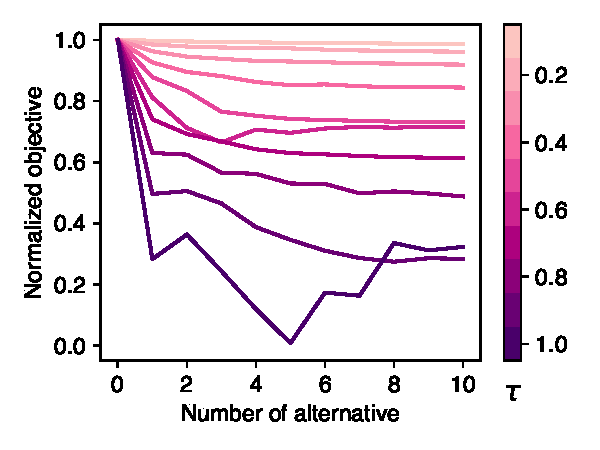
\includegraphics[width=0.99\columnwidth, trim=0 20 0 15, clip]{plots/impact-num-alternatives-train-objective-tau.pdf}
		\label{fig:impact-num-alternatives-train-objective-tau}
	}
	\hfill
	\subfloat[Test set.]{
		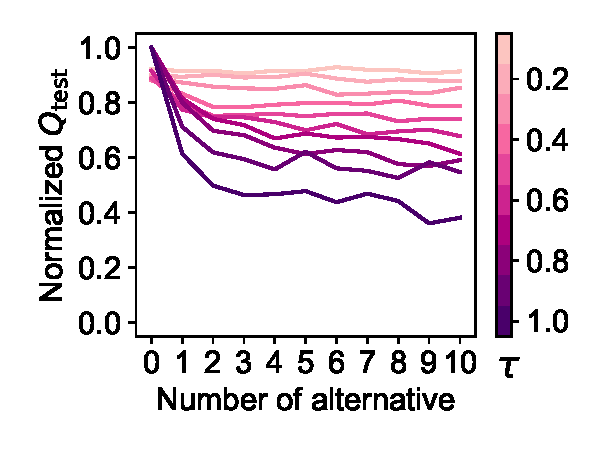
\includegraphics[width=0.99\columnwidth, trim=0 20 0 15, clip]{plots/impact-num-alternatives-test-objective-tau.pdf}
		\label{fig:impact-num-alternatives-test-objective-tau}
	}
	\caption{Median objective value $Q$, max-normalized per experimental setting, in sequential search, using \emph{MI} as feature selector and $k=10$.}
	\label{fig:impact-num-alternatives-objective-tau}
\end{figure*}

As we expected, the training-set objective value $Q$ of feature sets within a particular search run varies more for sequential search than for simultaneous search.
Figure~\ref{fig:impact-search-stddev-objective} visualizes this observation.
Also, the variance increases with the number of alternatives for sequential search, but decreases for simultaneous search.
I.e., simultaneous search finds relatively homogeneous feature sets, in particular, if many alternatives are desired.
However, on the test set, the variance also increases with the number of alternatives for simultaneous search.
This effect might be a result of overfitting.
Regarding test-set prediction performance, simultaneous search does not show lower variance than sequential search any more.

Surprisingly, the average feature-set quality of simultaneous search is not higher than for sequential search, neither regarding objective value $Q$ nor regarding prediction performance.
Figure~\ref{fig:impact-search-mean-objective} shows this behavior for the mean training-set objective of search runs.
Depending on the search setting, either of the two searches might yield better results.
An explanation for this phenomenon is that search results might be sub-optimal.
Exact optimization can time out, and \emph{Greedy Wrapper} uses a heuristic search per se.
As simultaneous search is harder than sequential search, it is affected more by timeouts.
In particular, 11.65\% of feature sets from simultaneous search were feasible but potentially sub-optimal, but no feature sets for sequential search.
The former figure strongly depends on the number of alternatives:
For up to three alternatives in simultaneous search, no or only a few feature sets are potentially sub-optimal, but 4\% of the feature sets for four alternatives and 35\% of the feature sets for five alternatives.
Based on these results, we focus on sequential search in the following.

\subsubsection{Number of Alternatives}

For sequential search, the training-set objective value $Q$ naturally decreases with the number of alternatives, at least for the feature-selection criteria optimized exactly.
Figure~\ref{fig:impact-num-alternatives-objective} illustrates this for \emph{MI}-based feature selection.
The other feature-selection methods, including the heuristic \emph{Greedy Wrapper}, exhibit similar effects.
As feature-set quality varies between datasets and number of features $k$, we apply normalization:
In Figure~\ref{fig:impact-num-alternatives-objective-max}, we have max-normalized the objective value for each search of alternatives, i.e., the highest objective value is scaled to~1.
This figure shows that there are multiple alternatives of similar quality, as the median feature-set quality remains relatively stable over the number of alternatives, and is close to the maximum.
Figure~\ref{fig:impact-num-alternatives-objective-min-max} uses min-max normalization, i.e., the worst of the alternatives gets~0 as objective.
This figure highlights that the training-set objective value decreases most from the original feature set to the first alternative, but less beyond.

Additionally, Figure~\ref{fig:impact-num-alternatives-objective} shows that the test-set objective value drops most to the first alternative as well.
However, the decrease in objective value over the alternatives is less visible than on the training set.
In particular, alternatives can even have a higher objective value than the original feature set, due to overfitting.
Similar findings hold for test-set prediction performance.
Thus, the alternative feature sets fulfill their purpose of being different solutions with similar quality.

Be aware that these observations refer to the quality of the found feature sets.
However, the more alternatives are desired, the more likely is an infeasible optimization problem.
For example, the \emph{MI} feature selector in sequential search always finds an original feature set, but the problem is infeasible in 2\% of the cases for the first alternative, 14\% for the second alternative, 24\% for the fifth alternative, and 30\% for the tenth alternative.
This outcome also depends on the dissimilarity, threshold $\tau$, which we analyze in the following.

\subsubsection{Dissimilarity Threshold}

As Figure~\ref{fig:impact-num-alternatives-objective-tau} shows for \emph{MI} as feature selector, the decrease of the objective value $Q$ over the number of alternatives can strongly depend on the dissimilarity threshold $\tau$.
For a low dissimilarity threshold, e.g., $\tau=0.1$, the objective value barely drops over the number of alternatives.
In contrast, for dissimilarity threshold, e.g, $\tau=1$, the objective decrease significantly.
This phenomenon also holds for test-set objective and test-set prediction performance, though the decrease with $\tau$ is less prominent.
Also, the the number of infeasible optimization problems, i.e., lack of valid alternative feature sets, increases with $\tau$.

While the previous observation were made for \emph{MI} as feature selector, they do not hold universally.
The results for \emph{Model Gain} strongly depend on $\tau$ as well, but the picture for \emph{FCBF} and \emph{Greedy Wrapper} is less clear.
In case of \emph{Greedy Wrapper}, this can be explained by its heuristic search.
In case of \emph{FCBF}, the fraction of infeasible solutions is much higher than for \emph{MI} in general, so adding further constraints has less impact.

\section{Conclusions and Future Work}
\label{sec:conclusion}

\balance % according to documentation, command might not work if issued to late in document, so hopefully placing it here suffices

\subsection{Conclusions}

Obtaining interpretable solutions is a highly active area of research in machine learning.
One way to foster interpretability is selecting a small set of features for predictions.
Traditional feature-selection methods yield \emph{one} feature set with high quality.
However, users might be interested in obtaining multiple, sufficiently different feature sets that, at the same time, have high quality.
Such alternative feature set might provide alternative explanations for predictions.

In this paper, we defined alternative feature selection as an optimization problem.
We formalized alternatives via constraints, independent from the feature-selection method.
Further, we presented approaches to solve the optimization problem for different categories of feature selection.
Finally, we ran an evaluation with 30 classification datasets and four feature-selection methods.
We varied a threshold for how strongly alternatives should differ from existing solutions.

In our experiments, we found that one can obtain alternative feature sets with similar quality as the original ones.
This worked with simultaneous search as well as sequential search for alternatives.
The latter procedure was significantly faster, and allows stopping the search once one does not want any more alternatives.
As expected, the quality of alternatives drops the more alternatives one desires and the more alternatives should differ.
The ultimate decision which trade-off between feature-set quality and alternatives is acceptable lies at the user.
Thus, we recommend evaluating different dissimilarity thresholds for alternatives.

\subsection{Future Work}

While our work introduced alternative feature selection, one might vary several points of our approach.
For example, one can integrate other feature-selection methods, in particular, embedded methods.
Further, one can vary the notion of alternatives, e.g., set-dissimilarity measure, definition for multiple alternatives, or soft constraints instead of hard constraints.
Finally, while our evaluation was domain-independent, the benefit of alternative feature set for explainable predictions should be analyzed in domain-specific case studies.

% \printbibliography
\bibliographystyle{IEEEtran}
\bibliography{IEEEabrv,references}

\end{document}
